\documentclass[11pt]{article}
\usepackage{geometry}                
\geometry{letterpaper}                   

\usepackage{graphicx}
\usepackage{amssymb}
\usepackage{epstopdf}
\usepackage{natbib}
\usepackage{amssymb, amsmath}
\usepackage{wrapfig}
\usepackage{empheq}




%\title{Title}
%\author{Name 1, Name 2}
%\date{date} 

\begin{document}



\section{Simulation results and discussion}
\subsection{Results of the SIR model}
All the values for the compartments s, x and r calculated by the model are within the possible intervals. Figure \ref{fig:mean_susceptible} and \ref{fig:mean_removed} show the mean over all districts for the susceptible and removed compartments respectively. One can see that the slope of the curve is steadier for the calculated model compared to the observed data. The observed curve of the infectious compartment in figure \ref{fig:mean_infectious} is highly nonlinear and the magnitude is slightly earlier than our calculated data. It is important to not only look at the means but the distribution of s, x and r within Haiti.\\

\begin{figure}[htb]
  %\centering
  \begin{minipage}[t]{0.49\textwidth}
    \centering
    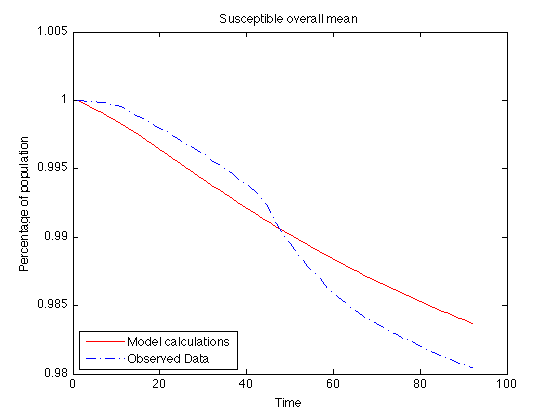
\includegraphics[width=\textwidth]{Bilder/susceptible_mean.png} 
    \caption{Mean over all districts for the susceptible compartment}
	\label{fig:mean_susceptible}
  \end{minipage}
  \hspace{0.02\textwidth}
  \begin{minipage}[t]{0.49\textwidth}
    \centering
    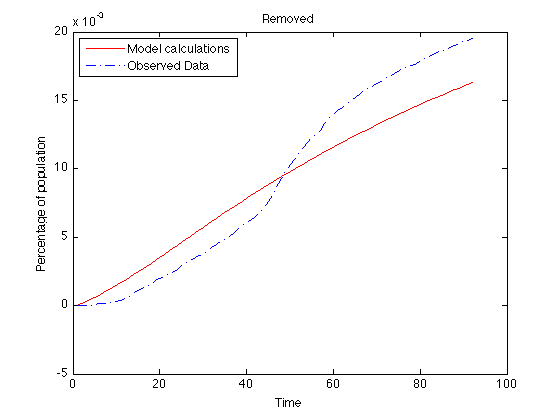
\includegraphics[width=\textwidth]{Bilder/removed_mean.png} 
    \caption{Mean over all districts for the removed compartment}
	\label{fig:mean_removed}
  \end{minipage}
\end{figure}



The plots \ref{fig:all_susceptible}, \ref{fig:all_removed} and \ref{fig:all_infectious} show the observed and calculated values of all ten compartments. The districts Nord, Nord-Est and Grand Anse show an incredible increase and decrease in the removed and susceptible compartments respectively. These compartments also have unlikely observed data for the infectious compartment as seen in figure \ref{fig:all_infectious}. In the district Grand Anse the amount of infected people decreses from  0.1\% to 0.04\% 



 



\begin{figure}[htb]
  %\centering
  \begin{minipage}[t]{0.49\textwidth}
    \centering
    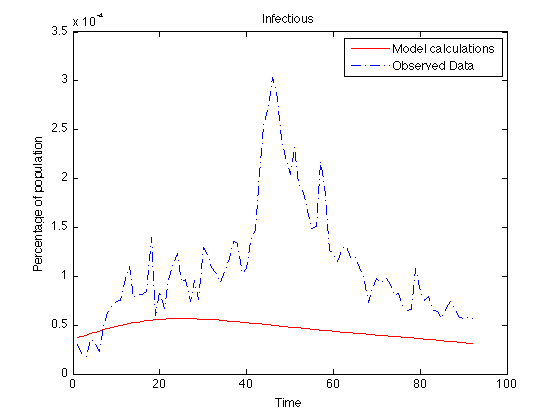
\includegraphics[width=\textwidth]{Bilder/infectious_mean.png} 
    \caption{Mean over all districts for the infectious compartment}
	\label{fig:mean_infectious}
  \end{minipage}
  \hspace{0.02\textwidth}
  \begin{minipage}[t]{0.49\textwidth}
    \centering
    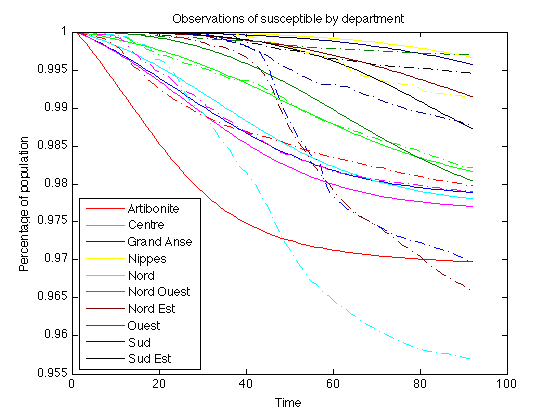
\includegraphics[width=\textwidth]{Bilder/susceptible.png} 
    \caption{Observed and calculated data for all districts of the susceptible compartment}
	\label{fig:all_susceptible}
  \end{minipage}
  
  \hspace{0.15\textwidth}

  %\centering
  \begin{minipage}[t]{0.49\textwidth}
    \centering
    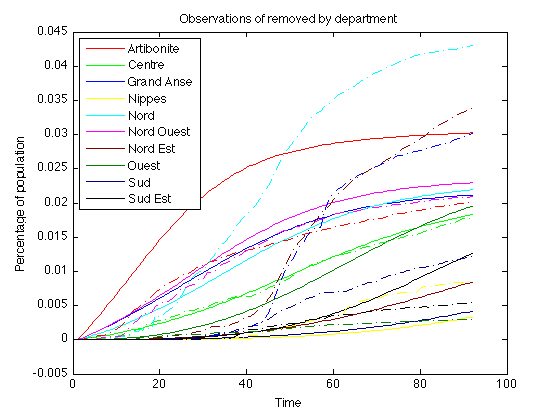
\includegraphics[width=\textwidth]{Bilder/removed.png} 
    \caption{Observed and calculated data for all districts of the removed compartment}
	\label{fig:all_removed}
  \end{minipage}
  \hspace{0.02\textwidth}
  \begin{minipage}[t]{0.49\textwidth}
    \centering
    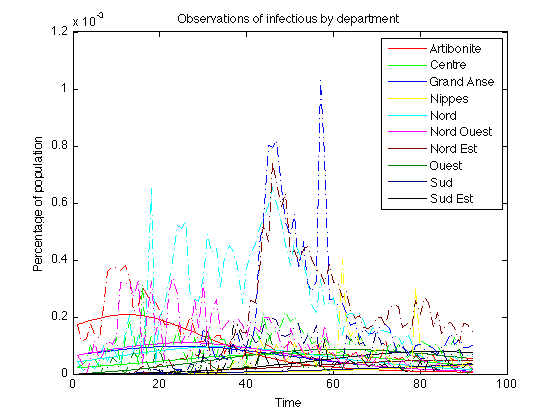
\includegraphics[width=\textwidth]{Bilder/infectious.png} 
    \caption{Observed and calculated data for all districts of the infectious compartment}
	\label{fig:all_infectious}
  \end{minipage}
\end{figure}




\end{document}